\documentclass[letterpaper]{article}
\usepackage{aaai}
\usepackage{times}
\usepackage{helvet}
\usepackage{courier}
\usepackage{amsmath}
\usepackage{amsfonts}
\usepackage{amssymb}
\usepackage{graphicx}
% %%%%%%%%%%%%%%%%%%%%%%%%%%%%%%%%%%%%%%%%%%%%%%%%%%%%%%
% PDFMARK for TeX and GhostScript
% Uncomment and complete the following for metadata if
% your paper is typeset using TeX and GhostScript (e.g
% if you use .ps or .eps files in your paper):
% \special{! /pdfmark where
% {pop} {userdict /pdfmark /cleartomark load put} ifelse
% [ /Author (John Doe, Jane Doe)
% /Title (Paper Title)
% /Keywords (AAAI, artificial intelligence)
% /DOCINFO pdfmark}
% %%%%%%%%%%%%%%%%%%%%%%%%%%%%%%%%%%%%%%%%%%%%%%%%%%%%%%
% PDFINFO for PDFTeX
% Uncomment and complete the following for metadata if
% your paper is typeset using PDFTeX
% \pdfinfo{
% /Title (Input Your Title Here)
% /Subject (Input The Proceedings Title Here)
% /Author (First Name, Last Name;
% First Name, Last Name;
% First Name, Last Name;)
% }
% %%%%%%%%%%%%%%%%%%%%%%%%%%%%%%%%%%%%%%%%%%%%%%%%%%%%%%
% Uncomment only if you need to use section numbers
% and change the 0 to a 1 or 2
% \setcounter{secnumdepth}{0}
% %%%%%%%%%%%%%%%%%%%%%%%%%%%%%%%%%%%%%%%%%%%%%%%%%%%%%%

\title{Divide-and-Evolve: the marriage of Descartes and Darwin\thanks{This work is being partially funded by Agence Nationale de la Recherche under research contract ANR-09-COSI-002-01}}
% Please leave SVN version number $Revision: 1131 $

%\author{Blind submission \#14}

\author{Johann Dr{\'e}o \ \ \ \ \ \ Pierre Sav{\'e}ant\\Thales Research \& Technology\\Palaiseau, France\\first.last@thalesgroup.com
\And Marc Schoenauer\\INRIA Saclay \& LRI\\Orsay, France\\marc.schoenauer@inria.fr
\And Vincent Vidal\\ONERA -- DCSD\\ Toulouse, France \\ Vincent.Vidal@onera.fr}


%\newcommand{\spread}{\linespread{0.8}}
\newcommand{\spread}{\linespread{1.0}}
\newcommand{\dae}{{\em Divide-and-Evolve}}
\newcommand{\DAEX}{{\sc DaE$_{\text{X}}$}}
\newcommand{\DAEYAHSP}{{\sc DaE$_{\text{YAHSP}}$}}
\newcommand{\YAHSP}{{\sc YAHSP}}

\begin{document}
\maketitle

\begin{abstract}
\DAEX, the concrete implementation of the \dae\ paradigm, is a domain-independent satisficing planning system based on Evolutionary Computation.
The basic principle is to carry out a {\em Divide-and-Conquer} strategy driven by an evolutionary algorithm.
The key components of \DAEX\ are a state-based decomposition principle, an evolutionary algorithm to drive the optimization process, and an embedded planner $X$ to solve the sub-problems.
The release that has been submitted to the competition is \DAEYAHSP, the instantiation of \DAEX\ with the
heuristic forward search \YAHSP\ planner.
The marriage of {\sc DaE} and \YAHSP\ matches a clean role separation:
\YAHSP\ gets a few tries to find a solution quickly whereas {\sc DaE} controls the optimization process.
\end{abstract}


\section{Introduction}
\DAEX, the concrete implementation of the \dae\ paradigm, is a
domain-independent satisficing planning system based on Evolutionary Computation
\cite{dae:evocop2006}. The basic principle is to carry out a {\em
Divide-and-Conquer} strategy driven by an evolutionary algorithm. The algorithm
is detailed in \cite{dae:icaps2010} and compared with state-of-the-art planners.
In order to solve a planning task ${\cal P}_D(I,G)$, the basic idea of \DAEX\ is
to find a sequence of goals $S_1, \ldots, S_n$, and to rely on an embedded
planner $X$ to solve the series of planning tasks ${\cal P}_D(S_{k},S_{k+1})$,
for $k \in [0,n]$ (with $S_0 = I$ and $S_{n+1} = G$). A \DAEX\ individual is thus a
sequence of goals which define a sequence of subproblems to be solved (a {\it
decomposition}). These subproblems are submitted successively to an embedded
planner $X$ and the global solution is obtained after the compression of these
intermediate solutions. The overall optimization process is controlled by
an evolutionary algorithm.

The decomposition principle of \DAEX\ is very general and could be applied to any type of planning tasks.
The scope of the planner is of course the one of the embbeded planner $X$. 
The release that has been submitted to the competition is \DAEYAHSP, the instantiation of \DAEX\ with the
heuristic forward search \YAHSP\ planner \cite{yahsp:icaps2004,yahsp:ipc:2011}.
The target is thus temporal satificing planning with conservative semantics, cost planning and classical STRIPS planning.
The marriage of {\sc DaE} and \YAHSP\ matches a clean role separation:
\YAHSP\ gets a few tries to find a solution quickly whereas {\sc DaE} controls the optimization process.
In the current release we have introduced an initial estimation processing of the maximum number of tries allowed to YAHSP for all individual evaluations.
This parameter is crucial for the time consumption of the algoritm.

\section{The Evolutionary Engine}

\begin{figure}[h]
\hskip -1cm
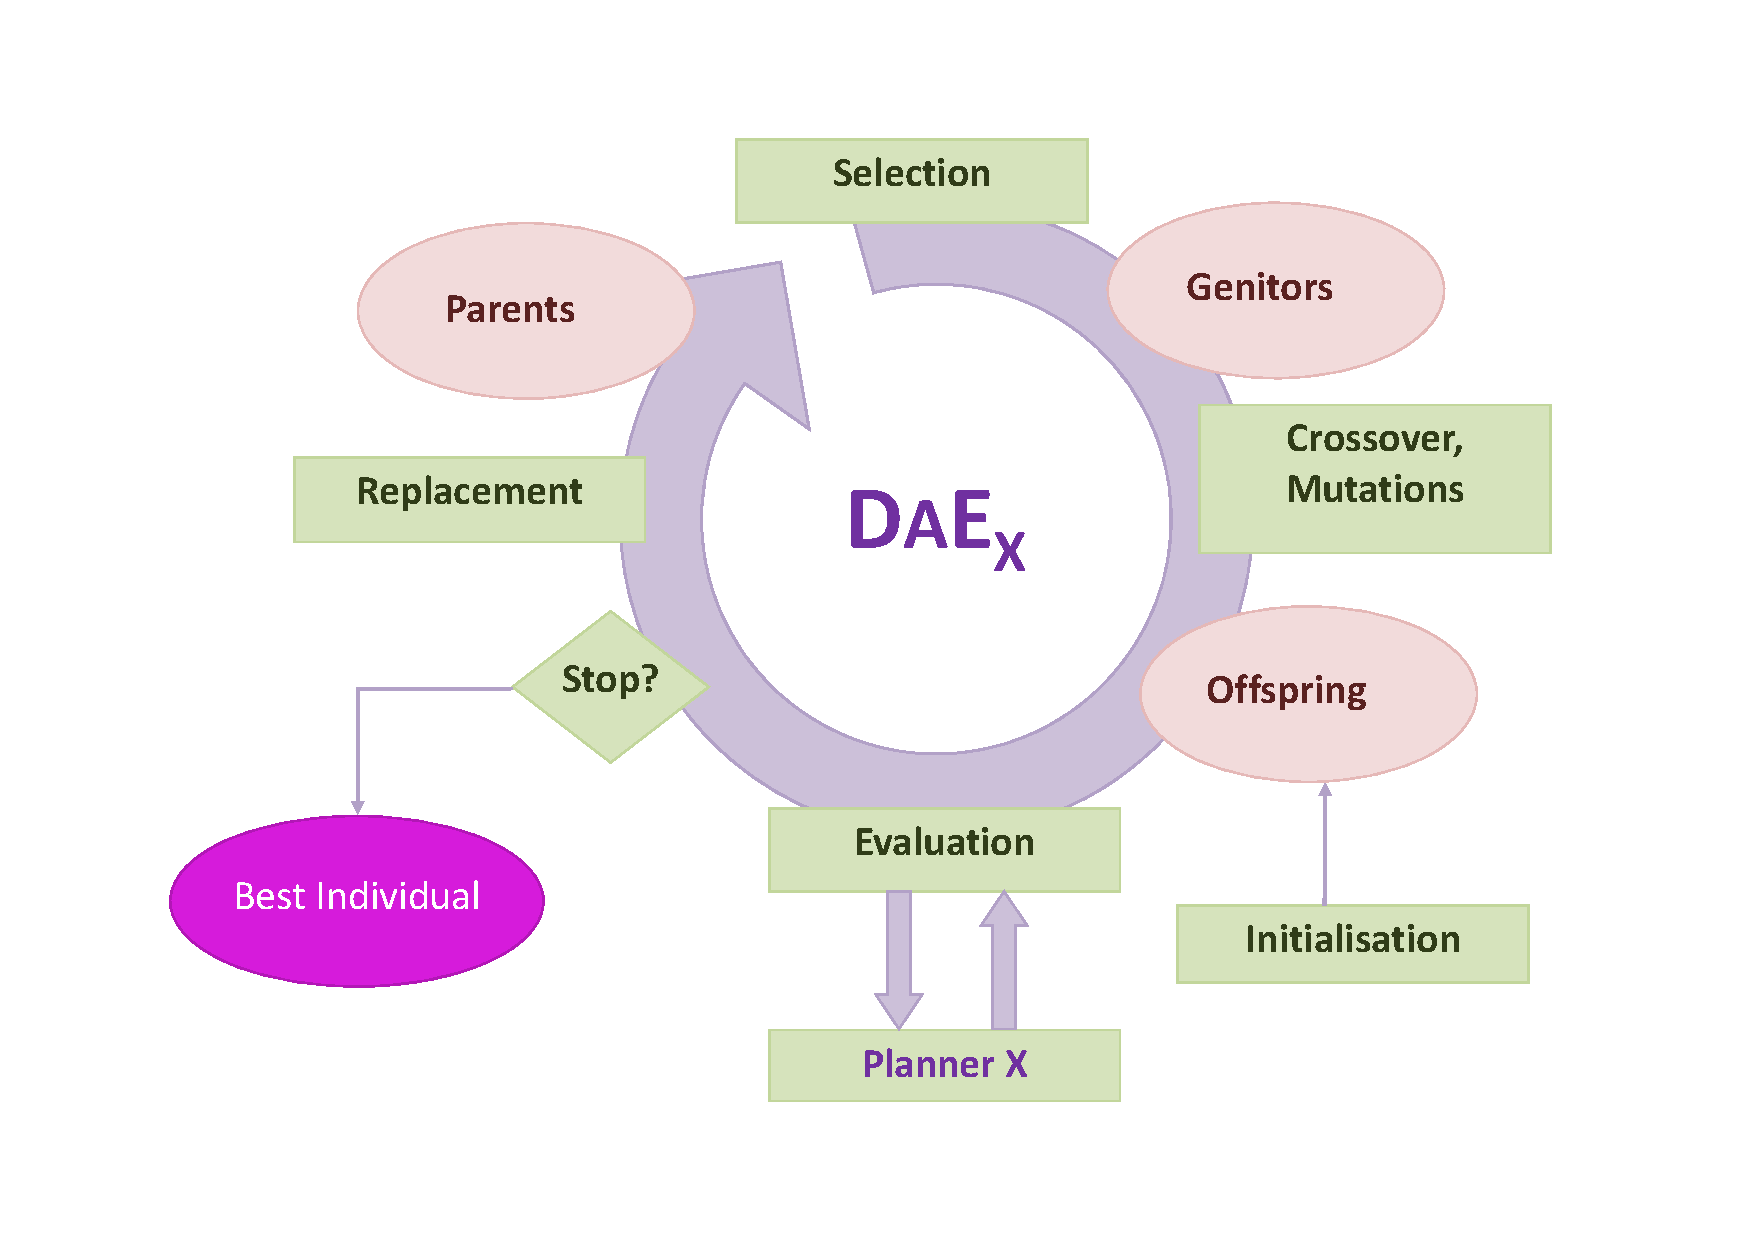
\includegraphics[width=0.6\textwidth]{DAE.pdf}
%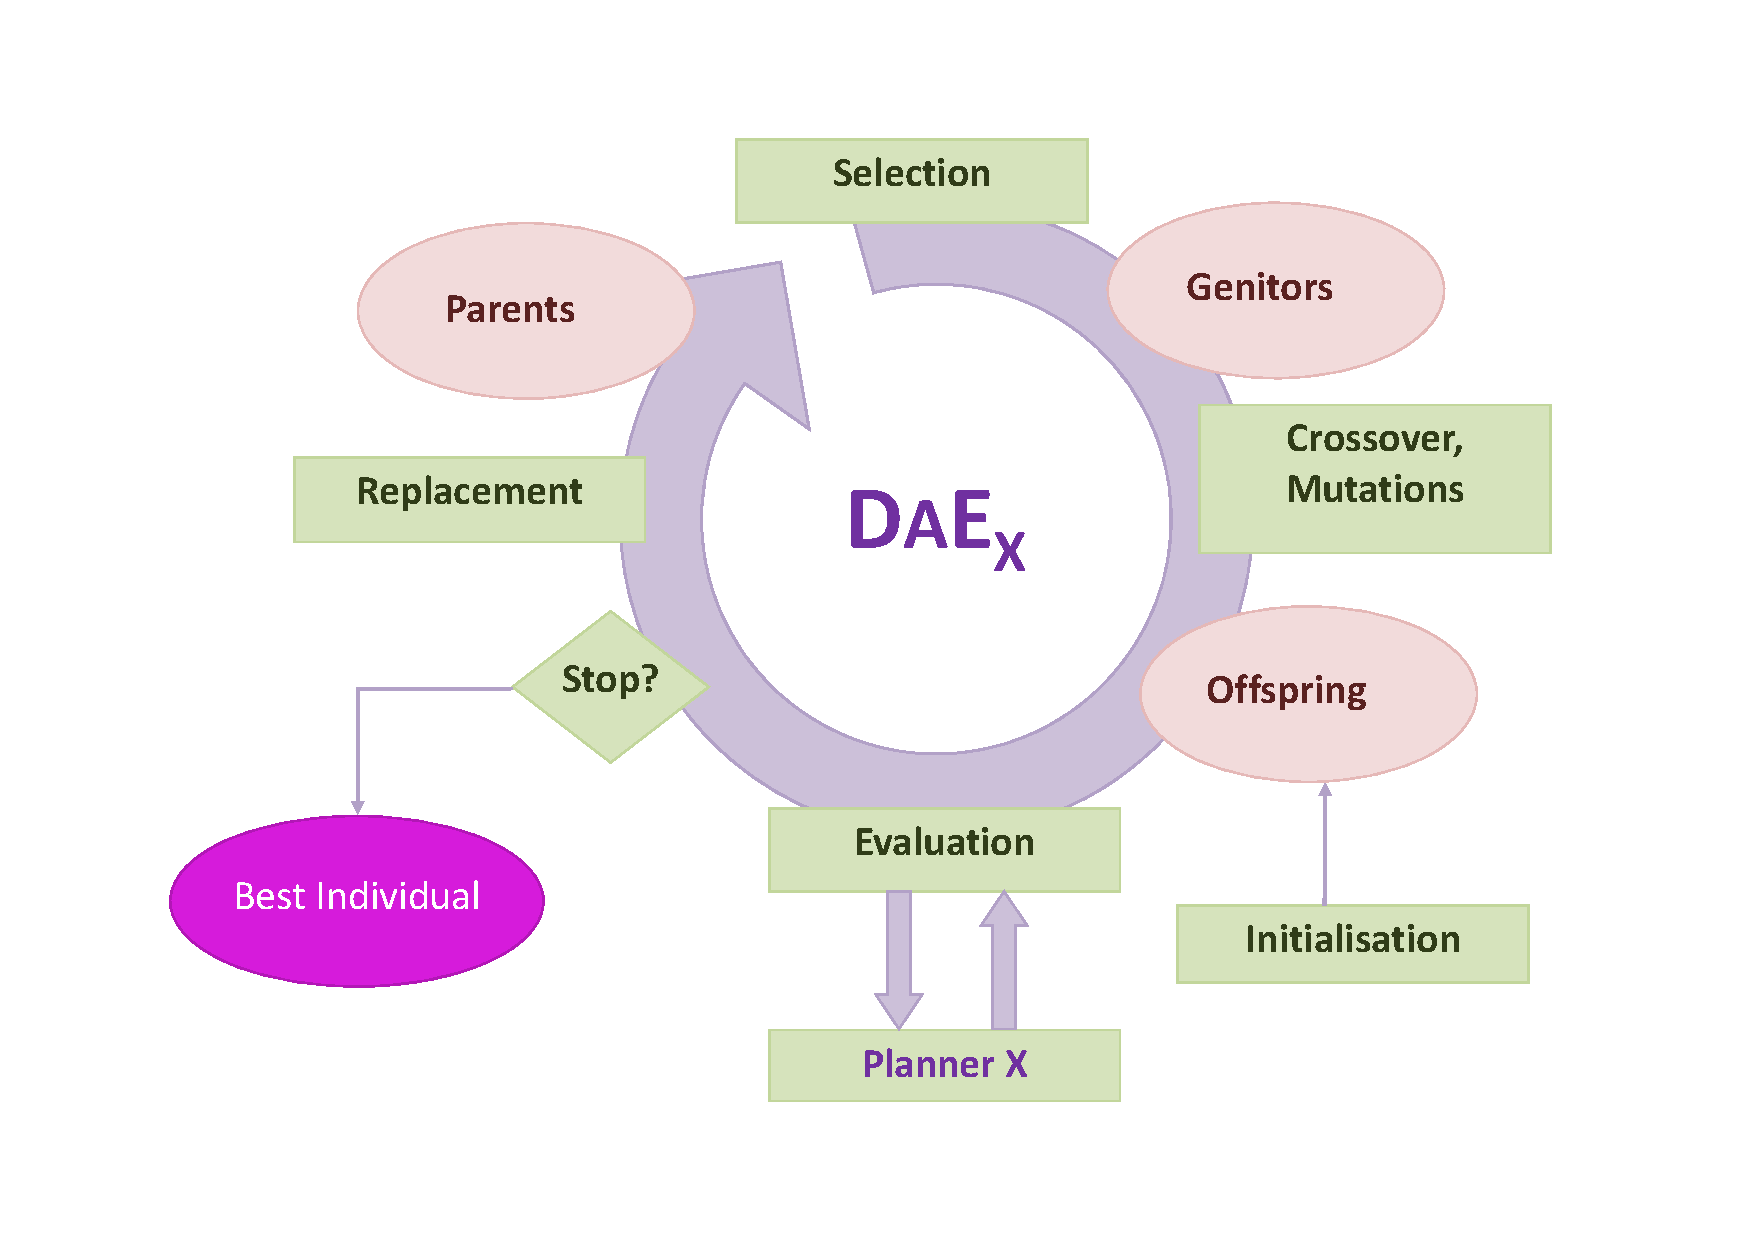
\includegraphics[width=10cm]{DAE.pdf}
\vskip -0.5cm
\caption{The standard evolutionary loop}
\label{fig:daeloop1}
\end{figure}

Figure \ref{fig:daeloop1} depicts the standard evolutionary loop which mimics a biological evolution.
The fitness implements a gradient towards feasibility for unfeasible individuals
and a gradient towards optimality for feasible individuals. Feasible individuals
are always preferred to unfeasible ones. Population initialization as well as
variation operators are driven by the critical path $h^1$ heuristic
\cite{h1:aips2000} in order to discard inconsistent state orderings, and atom
mutual exclusivity inference in order to discard inconsistent states. Beside a
standard one-point crossover for variable length representations, four mutations
have been defined: addition (resp. removal) of a goal in a sequence, addition
(resp. removal) of an atom in a goal. The selection is a comparison-based
deterministic tournament of size 5.

% Parameter tuning
For the sequential release, Darwinian-related parameters of \DAEX\ have been
fixed after some early experiments \cite{dae:evocop2006} whereas parameters
related to the variation operators have been tuned using the Racing method
\cite{dae:gecco2010}.



We added two novelties to the version described in
\cite{dae:icaps2010}. One important parameter is the maximum number of expanded
nodes allowed to the \YAHSP\ sub-solver which defines empirically what is
considered as an easy problem for \YAHSP. As a matter of fact, the minimum
number of required nodes varies from few nodes to thousands depending of the
planning task. In the current release this number is estimated during the
population initialization stage. An incremental loop is performed until the
ratio of feasible individuals is over a given threshold or a maximum boundary has
been reached. By default this number is doubled at each iteration until at least
one feasible individual is produced or 100000 has been reached.

Furthermore we add the capability to perform restarts within a time contract in
order to increase solution quality.

The fitness used for the competition differs from the one described in \cite{dae:icaps2010}.
The fitness for bad individuals has been simplified by withdrawing the Hamming distance to the goal.
The new fitness depends only on the ``decomposition distance'': the number of intermediate goals reached and more specifically the one that are ``useful''.
A useful intermediate goal is a goal that require a non-empty plan to be reached.




% the number of remaining goals to solve in the sequence.

% d�compositions dont la taille d�passe la longueur max lmax
%return _fitness_penalty * ((double)_l_max + 1.0) * (double)_l_max * (double)_unknown_parameter * 2; 

% echec avant la derni�re station
%return _fitness_penalty * ((double)_l_max -(double)decompo.get_number_useful_goals() + 1.0) * (double)_l_max * (double)_unknown_parameter;

% Echec � la derni�re station
%return _fitness_penalty * ((double)_l_max -(double)decompo.get_number_useful_goals() + 1.0); }



\section{Conclusion}

\bibliographystyle{aaai}
\bibliography{dae_mt}


\end{document}





